% !TEX root = ../paper.tex
%http://sphweb.bumc.bu.edu/otlt/MPH-Modules/BS/BS704_HypothesisTesting-ANOVA/BS704_HypothesisTesting-Anova_print.html
\section{Results}
We will now present the results that we achieved through out our experiment and also how they were achieved. We will first present our findings in respect to success rate(based on hit success), then in respect to efficiency(based on time per target), and finally in respect to accuracy(based on distance to target). Finally, we will look at the questionnaires and show the significant findings there in terms of ease of use. We will discuss these results later, in the \nameref{sec:discussion} section.  
Each of the four interaction techniques, \pinch, \swipe, \throw and \tilt were completed 18 times per participant. 
For each grid size, each technique was performed 477 times. 

\subsection{Success Rate}
In this section we will present the results related to the success of hitting a target.
We will perform an analysis of the success rate and the effect of each technique with respect to grid sizes.

The success rate's mean and standard deviation, M(St.D.) for each technique for small(S) and large(L) grid size can be seen in \Cref{tab:meanHitTechnique} and in \Cref{fig:successResults} the results are shown as a graph.

\begin{table}[H]
	\centering
	\textbf{Success Hit Means}\\[4pt]
	\begin{adjustbox}{width=\columnwidth}
	\begin{tabular}{|c|c|c|c|c|}
			\hline
			\rowcolor[HTML]{9B9B9B} 
			& \textbf{Pinch} & \textbf{Swipe} & \textbf{Throw} & \textbf{Tilt} \\
			\rowcolor[HTML]{9B9B9B} 
			 & (n = 477) & (n = 477) & (n = 477) & (n = 477) \\ \hline
			S & 0.65 (0.48)       & 0.91 (0.29)         & 0.83 (0.37)         & 0.58 (0.49)        \\ \hline
			L & 0.78 (0.41)        & 0.97 (0.18)         & 0.94 (0.25)        & 0.78 (0.41)       \\ \hline
	\end{tabular}
	\end{adjustbox}
	\caption{Mean hit  and standard deviation for each technique per target for small(S) and large(L) grid.}
	\label{tab:meanHitTechnique}
\end{table}

\begin{figure}[H]
	{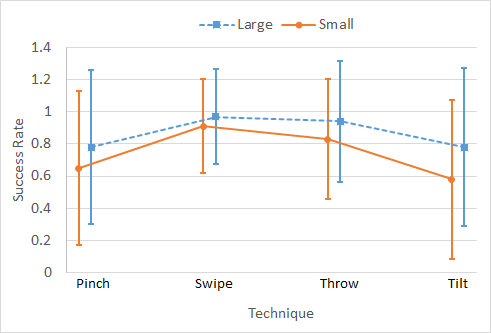
\includegraphics[width = 1\columnwidth ]{images/success.png}} 
	\caption{
		Mean and standard deviation for each technique in regards to hit rate per target.
	}
	\label{fig:successResults}
\end{figure}

In order to see the effect of each technique on the hit ratio per target for the different grid sizes, we performed two different one-way ANOVA's, where we split the data between the two different grid sizes.
We then performed a post-hoc pairwise LSD test to see where the significant difference were.
 
For the the small grid, we got $(p<0.001)$, $(F(2.722, 1295.674)=62.754)$, (Greenhouse-Geisser correction: 0.907).
The pairwise test showed that all techniques were significantly different. \pinch and \swipe had $(p < 0.001)$, \pinch and \throw $(p <0.001)$, \pinch and \tilt $(p = 0.031)$, \swipe and \throw $(p=0.001)$, \swipe and \tilt $(p < 0.001)$ and finally, \throw and \tilt had $(p<0.001)$. 

For the large grid, we got $(p<0.001)$, $(F(2.472, 1176.749)=42.773)$, (Greenhouse-Geisser correction: 0.824).
The pairwise test showed that all of the techniques, with the exception of \pinch and \tilt, were statistically different from each other. The results were as following: \pinch and \swipe $(p<0.001)$, \pinch and \throw $(p<0.001)$, \pinch and \tilt $(p=1.000)$, \swipe and \throw $(p=0.025)$, \swipe and \tilt $(p<0.001)$, and finally \throw and \tilt $(p<0.001)$.

\subsection{Efficiency}
In this section we present the efficiency results which defines the amount of time spent performing a technique.
We perform an analysis of the efficiency and the effect of each technique with respect to grid sizes.

\Cref{tab:meanTimesTechnique} shows the mean time per target in seconds for each of the techniques as well as their standard deviation for both grid sizes. 
\begin{table}[H]
	\centering
	\textbf{Time Means}\\[4pt]
	\begin{adjustbox}{width=\columnwidth}
	\begin{tabular}{|c|c|c|c|c|}
		\hline
		\rowcolor[HTML]{9B9B9B} 
		 & \textbf{Pinch} & \textbf{Swipe} & \textbf{Throw} & \textbf{Tilt} \\ 
		 \rowcolor[HTML]{9B9B9B} 
		 & (n = 477) & (n = 477) & (n = 477) & (n = 477) \\ \hline
		S & 9.23 (6.48)          & 6.41  (4.49)         & 7.73 (6.60)          & 6.67 (4.49)  \\ \hline
		L & 8.09 (6.60)          & 5.01  (2.66)          & 6.42 (5.43)          & 5.33 (3.04) \\ \hline
	\end{tabular}
	\end{adjustbox}
	\caption{Mean time and standard deviation for each technique per target for small(S) and large(L) grid.}
	\label{tab:meanTimesTechnique}
\end{table}

\begin{figure}[H]
	{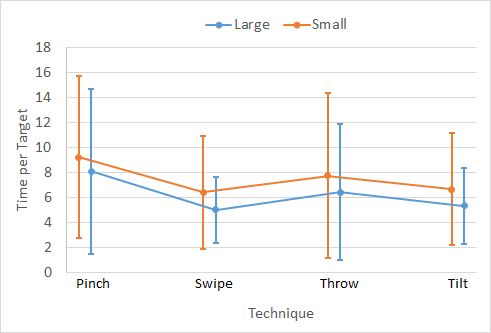
\includegraphics[width = 1\columnwidth ]{images/time.png}} 
	\caption{
		Mean and standard deviation for each technique in regards to time per target.
	}
	\label{fig:timeResults}
\end{figure}

To get the effect of each technique on the time for the different grid sizes, we performed two one-way ANOVA's, one for the small grid and another for the large grid.
A post-hoc pairwise LSD test to see where the significant difference were.

For the the small grid, we got $(p<0.001)$, $(F(2.740, 1304.290)=26.523)$, (Greenhouse-Geisser correction: 0.913).
The pairwise test showed that all techniques were significantly different except \swipe and \tilt. 
\pinch and \swipe had $(p < 0.001)$, 
\pinch and \throw $(p <0.001)$, 
\pinch and \tilt $(p < 0.001)$, 
\swipe and \throw $(p < 0.001)$, 
\swipe and \tilt $(p = 0.354)$ and finally, 
\throw and \tilt had $(p = 0.004)$. 

For the large grid, we got $(p<0.001)$, $(F(2.221, 1057.144)=44.539)$, (Greenhouse-Geisser correction: 0.740).
The pairwise test showed that all of the techniques, with the exception of \swipe and \tilt, were statistically different from each other. The results were as following: 
\pinch and \swipe $(p<0.001)$, 
\pinch and \throw $(p<0.001)$, 
\pinch and \tilt $(p<0.001)$, 
\swipe and \throw $(p<0.001)$, 
\swipe and \tilt $(p=0.077)$, and finally 
\throw and \tilt $(p<0.001)$.

\subsection{Accuracy}
Finally, we will perform an analysis of the accuracy and the effect of each technique with respect to grid sizes.
Here, we took three different measures of accuracy; the distance between where the user hit and the target cell as well as taking the $x$ and $y$ axis independently. 
These were all measured in pixels.
This was because there were signs that certain techniques might miss in a specific direction, and we wanted to see if the data supported that. 
An overview of the distance mean and standard deviation in pixels can be seen in \Cref{tab:distance} and \Cref{fig:distanceResults}.

\begin{figure}[H]
	{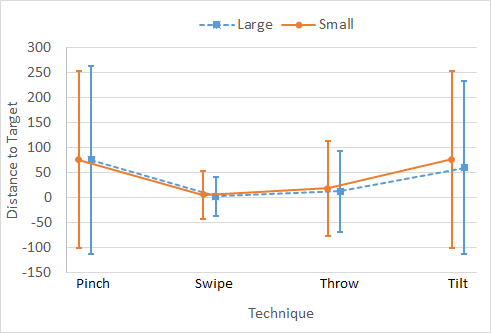
\includegraphics[width = 1\columnwidth ]{images/distance.png}} 
	\caption{
		Mean and standard deviation for each technique in regards to distance.
	}
	\label{fig:distanceResults}
\end{figure}

\begin{table}[H]
	\centering
	\textbf{Distance Means}\\[4pt]
	\begin{adjustbox}{width=\columnwidth}
	\begin{tabular}{|c|c|c|c|c|}
		\hline
		\rowcolor[HTML]{9B9B9B} 
		& \textbf{Pinch} & \textbf{Swipe} & \textbf{Throw} & \textbf{Tilt} \\
		\rowcolor[HTML]{9B9B9B} 
		& (n = 477) & (n = 477) & (n = 477) & (n = 477) \\ \hline
		S & 75.97 (176.15) & 5.40 (47.81) & 18.60 (95.29)  & 76.51  (177.45) \\ \hline
		L & 75.41 (187.58) & 2.29 (38.82) & 12.37 (81.36) & 59.88 (172.22) \\ \hline
	\end{tabular}
	\end{adjustbox}
	\caption{Mean and standard deviation for the distance for each technique per target for small(S) and large(L) grid.}
	\label{tab:distance}
\end{table}

We performed two one way ANOVA's, one for each grid size, on the distance data.

For the the small grid, we got $(p<0.001)$, $(F(2.341, 1114.249)=37.504)$, (Greenhouse-Geisser correction: 0.780).
The pairwise test showed that all techniques were significantly different except \pinch and \tilt. 
\pinch and \swipe had $(p < 0.001)$, 
\pinch and \throw $(p <0.001)$, 
\pinch and \tilt $(p = 0.961)$, 
\swipe and \throw $(p = 0.008)$, 
\swipe and \tilt $(p < 0.001)$ and finally, 
\throw and \tilt had $(p < 0.001)$. 

For the large grid, we got $(p<0.001)$, $(F(2.176, 1036.004)=33.315)$, (Greenhouse-Geisser correction: 0.725).
The pairwise test showed that all of the techniques, with the exception of \pinch and \tilt, were statistically different from each other. The results were as following: 
\pinch and \swipe had $(p < 0.001)$, 
\pinch and \throw $(p <0.001)$, 
\pinch and \tilt $(p = 0.171)$, 
\swipe and \throw $(p = 0.015)$, 
\swipe and \tilt $(p < 0.001)$ and finally, 
\throw and \tilt had $(p < 0.001)$. 

\begin{table}[H]
	\centering
	\textbf{X and Y Distance Means}\\[4pt]
	\begin{adjustbox}{width=\columnwidth}
	\begin{tabular}{|c|c|c|c|c|}
		\hline
		\rowcolor[HTML]{9B9B9B} 
		& \textbf{Pinch} & \textbf{Swipe} & \textbf{Throw} & \textbf{Tilt} \\
		\rowcolor[HTML]{9B9B9B} 
		& (n = 477) & (n = 477) & (n = 477) & (n = 477) \\ \hline
		S XD. & 54.33 (140.87) & 3.78 (40.15) & 10.32 (81.84) & 49.23 (151.36) \\ \hline
		L XD. & 55.32 (159.88) & 1.88 (31.74) & 10.32 (74.01) & 49.23 (157.35) \\ \hline
		S YD. & 42.90 (110.30) & 2.00 (26.16) & 8.00 (49.37) & 39.3 (99.82)3 \\ \hline
		L YD. & 37.41 (104.18) & 1.14 (22.37) & 4.33 (34.21) & 22.86 (73.75) \\ \hline
	\end{tabular}
	\end{adjustbox}
	\caption{Mean and standard deviation for distance on the X-Axis(XD) and distance on the Y-Axis(YD) for each technique per target for small(S) and large(L) grid.}
	\label{tab:distanceXY}
\end{table}

\begin{figure}[H]
	{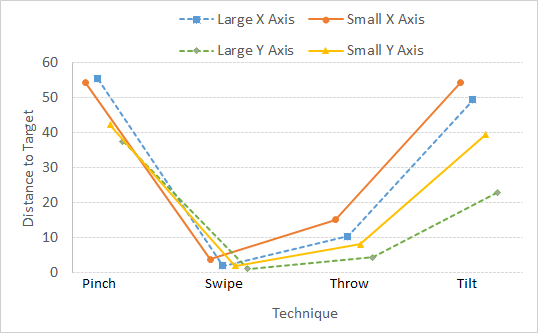
\includegraphics[width = 1\columnwidth ]{images/distance_axis.png}} 
	\caption{
		Mean and standard deviation for each technique in regards distance on the x-axis and y-axis.
	}
	\label{fig:distanceXYResults}
\end{figure}

To get a better understanding of the distance we decided to examine the distance in regards to the x-axis and in regards to the y-axis.
The results can be seen in \Cref{tab:distanceXY} and \Cref{fig:distanceXYResults}

\todo[inline]{Jeni: Should we include the numbers from the SPSS analysis of the X-distance and Y-distance data?}

%We then performed a post hoc LSD test to see where the significant differences were located. 
